\documentclass[conference]{IEEEtran}
\usepackage[T1]{fontenc}
\usepackage[utf8]{inputenc}
\usepackage{amsmath,amssymb}
\usepackage{booktabs}
\usepackage{graphicx}
\usepackage{tikz}
\usetikzlibrary{arrows.meta,positioning,fit,calc}
\usepackage{microtype}
\usepackage{xcolor}
\usepackage[hidelinks]{hyperref}
\usepackage{siunitx}
\sisetup{group-separator={,},group-minimum-digits=4,detect-weight=true}
\newcommand{\rsr}{\operatorname{rsr}}
\newcommand{\sat}{\operatorname{sat}}
\newcommand{\code}[1]{\texttt{#1}}

%% ---- synthesis numbers (filled from Yosys/ABC on the ASAP7 TT RVT libraries) ----
\newcommand{\areaLogicTotal}{TBD}
\newcommand{\fmaxSA}{TBD}
\newcommand{\fmaxAll}{TBD}
\newcommand{\synthRows}{SystolicArray & TBD & TBD & TBD & TBD \\}
\newcommand{\synthDiscussion}{TBD.}


\begin{document}

\title{whisper-si: A Bit-Exact Integer Whisper-tiny Accelerator\\Generated in Chisel with Weights in the Source Tree}

\author{\IEEEauthorblockN{Rachit Tibrewal}
\IEEEauthorblockA{\code{github.com/tibrewalrachit/wispr-on-chip}}}

\maketitle

\begin{abstract}
We present whisper-si, a complete hardware implementation of OpenAI's Whisper-tiny automatic speech recogniser (37.2\,M parameters) written as a Chisel generator. The design executes the whole model on one chip: a $32\times32$ int8 weight-stationary matmul engine, a 16-lane vector unit, an attention unit with online softmax over 64-key tiles, a KV cache, a streaming argmax sampler, and a sequencer that executes a 186-instruction micro-program generated from the model graph. All 247 weight tensors are committed to the repository as hex text (\SI{38.5}{MB}) and consumed at elaboration time through one of three interchangeable ROM/SRAM backends. Correctness is defined by an integer golden model in numpy: the RTL is correct if and only if it reproduces the same bits. We show that this holds on 35 full-context Verilator runs over 24 real audio clips, with every token identical to the golden model, and that the integer model meets a word-error-rate gate against the fp32 reference (\SI{5.52}{\percent} vs.\ \SI{5.54}{\percent} on 200 LibriSpeech utterances; \SI{7.58}{\percent} vs.\ \SI{8.08}{\percent} on the 20 utterances run on the RTL). An analytic cycle model built only from unit-level measurements predicts every end-to-end run within \SI{0.2}{\percent}. Logic synthesis of the compute blocks on the ASAP7 \SI{7}{nm} predictive PDK gives \areaLogicTotal\,mm$^2$ of standard cells; the systolic array closes at \fmaxSA\ and the design as a whole at \fmaxAll, and at \SI{1}{GHz} a \SI{30}{s} window is transcribed in \SI{42}{ms} plus \SI{0.2}{ms} per generated token.
\end{abstract}

\section{Introduction}
Whisper~\cite{whisper} is the de facto open speech recogniser, and its smallest variant, Whisper-tiny, is an attractive target for a dedicated accelerator: 4 encoder and 4 decoder layers of width 384 with 6 heads, small enough that the entire weight set can live on chip. Building such an accelerator raises three questions that this paper answers with a working design rather than a proposal. \emph{(i)} Which integer numerics let an int8 datapath match the fp32 model's accuracy? \emph{(ii)} How can a Verilator simulation of the chip be checked against real audio without any tolerance? \emph{(iii)} What does the resulting design cost in cycles and, on a \SI{7}{nm} process, in area and clock rate?

Our contributions are:
\begin{itemize}
\item A frozen integer specification of Whisper-tiny (Section~\ref{sec:numerics}) whose executable form, a numpy model, is both the accuracy vehicle and the source of every RTL test vector.
\item A Chisel generator (Section~\ref{sec:arch}) in which the model graph is compiled to a micro-program at generation time, and in which weights are ordinary source files hashed and consumed at elaboration.
\item A verification ladder (Section~\ref{sec:verif}) from single ops to whole clips in which every level is bit-exact, plus a breakpoint mechanism that locates chip-level divergences by binary search over the micro-program.
\item Measured performance (Section~\ref{sec:perf}): cycle counts, an analytic model that reproduces them, and ASAP7 synthesis results at a \SI{1}{GHz} target.
\end{itemize}
The complete source, weights, references and status reports are in the repository; every number in this paper is reproducible with the \code{Makefile} targets listed in Section~\ref{sec:repro}.

\section{Method: the golden model is the specification}
The project ran in five phases, each ending with a commit and a dated status entry; design choices that deviate from the original brief are numbered decisions in \code{docs/decisions.md}. The central rule is that numerics are frozen in Python before any RTL exists. \code{golden/whisper\_int.py} is a complete integer implementation of Whisper-tiny: it takes an int8 log-mel spectrogram and produces token ids using only integer multiplies, shifts, saturations and table lookups. The only floating-point code is the weight generator, which turns the fp16 checkpoint plus calibration statistics into int8 weights, int32 multipliers and shift amounts.

Because the golden model is executable it doubles as the vector generator: every RTL unit test loads tensors dumped by it, and the end-to-end test compares the RTL token stream with the golden token stream. Accuracy is checked once, at the golden level, against openai-whisper's own greedy decoder run on the CPU over a single \SI{30}{s} window; the fp32 references regenerate byte-identically and agree with the HuggingFace weights to zero difference on 60 clips. The gate is that the integer model's WER may exceed fp32 by at most 0.5 points absolute on 200 LibriSpeech test-clean utterances~\cite{librispeech}; it passes at \SI{5.52}{\percent} versus \SI{5.54}{\percent}.

\section{Numerics}\label{sec:numerics}
Throughout, $\rsr(x,s)=(x+2^{s-1})\gg s$ and $\sat_W$ clamps to $W$-bit two's complement; every rounding and saturation is explicit and there is no tolerance anywhere. Table~\ref{tab:formats} lists the tensor formats.

\begin{table}[t]
\caption{Activation formats. ``Static'' scales come from calibration on 128 dev-clean utterances; ``dynamic'' scales are per token.}
\label{tab:formats}
\centering\small
\begin{tabular}{@{}lll@{}}
\toprule
Tensor & Format & Scale \\
\midrule
mel input & int8 & static \\
conv outputs, residual stream & int16 & static per point \\
LayerNorm output & int16, $2^{-F}$ & transient \\
matmul inputs & int8 & dynamic per token \\
Q, K & int8 & static per head \\
V & int8 & static per tensor \\
attention output & int16 & $O/l\cdot 2^{7}$ \\
fc1 output (GELU input) & int16 & static \\
LM-head logits & int32 & wide mode \\
\bottomrule
\end{tabular}
\end{table}

\paragraph{Matmul inputs and edge requantisation} Weights are int8, symmetric, per output channel. Matmul inputs are int8 with a per-token dynamic scale: for each row the vector unit finds $m=\max|x_{16}|$, computes $r=\lfloor(127\cdot2^{16}+m/2)/m\rfloor$ and quantises $a_8=\sat_8(\rsr(x_{16}\,r,16))$. The row's $m$ travels with the tile as a \emph{row factor} so the matmul drain can undo it:
\begin{align}
t &= \sat_{40}\big(\rsr(\mathrm{acc}\cdot M[n],\,s_1)\big),\\
y &= \sat_W\big(\rsr(t\cdot \mathrm{rowfac}[m] + (B[n]\ll(s_2-16)),\,s_2)\big),
\end{align}
with $s_2=24$ for int8 and $20$ for int16 outputs. A wide mode keeps int32 logits for the LM head.

\paragraph{Residual stream} Calibration shows encoder residual maxima of 274 against channel medians of 5.8 (Whisper's well-known outlier channels~\cite{llmint8}). An int8 residual leaves typical values 0--2 LSBs and yields \SI{98}{\percent} WER, so the residual is int16 (decision~5); int8 remains a configuration option.

\paragraph{LayerNorm} uses an integer mean $\rsr(\Sigma x\cdot 5592405,23)$ (i.e.\ $\Sigma x\cdot2^8/384$), a variance from $\Sigma x^2$, a 256-entry inverse-square-root table on the normalised mantissa followed by one Newton step, and per-channel gain and bias folded into the output scale.

\paragraph{GELU} is computed as $x\cdot\Phi(x)$ on the int16 fc1 output with a 256-entry $\Phi$ table and linear interpolation (decision~6). The alternative int8$\to$int8 table, with fc1 maxima of 326 against medians of 14, costs \SI{21}{\percent} WER.

\paragraph{Attention} Q and K use static per-head scales and V a per-tensor scale, since per-token scales cannot be factored out of the softmax. Scores $s=q_8\cdot k_8$ are processed in key tiles of 64 with an online softmax~\cite{onlinesoftmax}: a running maximum $m_x$, distances $d=\min(4095,\rsr((m_x-s)M_q,s_q))$, a Q1.15 exponential table $E(d)$ with 16-point interpolation, a rescale by $\alpha=E(\Delta m)$ when the maximum grows, and a 36-bit accumulator $O\mathrel{+}=\Sigma_j p_j v_j$. After the last tile a pipelined divider forms $r_l=\lfloor(2^{40}+l/2)/l\rfloor$ and the output is $\sat_{16}(\rsr(O\,r_l,33))$.

\paragraph{Decoding} replicates Whisper's greedy rules exactly: a four-token prompt, sampling from position~3, suppression of 88 non-speech tokens (plus blank and end-of-text on the first step), lowest-index argmax, and a stop at end-of-text or 224 tokens.

\section{Architecture}\label{sec:arch}
\begin{figure}[t]
\centering
\resizebox{\columnwidth}{!}{%
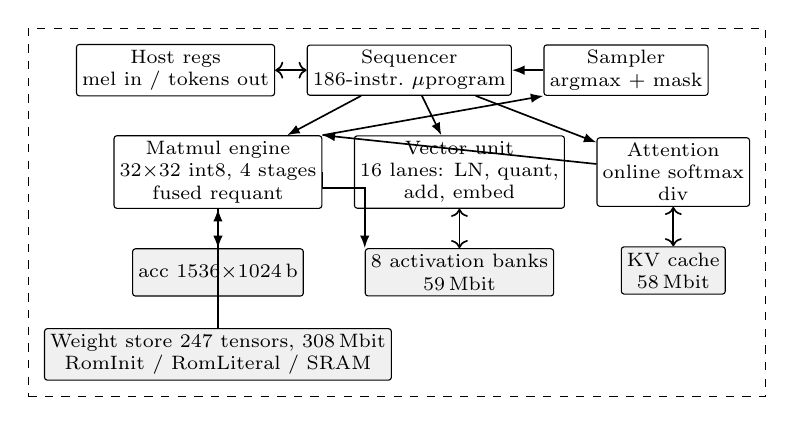
\begin{tikzpicture}[
  blk/.style={draw,rounded corners=1pt,minimum height=6mm,inner sep=2pt,font=\scriptsize,align=center},
  mem/.style={blk,fill=black!6},
  arr/.style={-{Latex[length=1.6mm]},semithick},
  node distance=3mm and 4mm]
\node[blk] (seq) {Sequencer\\186-instr.\ $\mu$program};
\node[blk,below left=5mm and -2mm of seq] (eng) {Matmul engine\\$32{\times}32$ int8, 4 stages\\fused requant};
\node[blk,right=of eng] (vu) {Vector unit\\16 lanes: LN, quant,\\add, embed};
\node[blk,right=of vu] (att) {Attention\\online softmax\\div};
\node[mem,below=5mm of eng] (acc) {acc 1536$\times$1024\,b};
\node[mem,below=5mm of vu] (banks) {8 activation banks\\\SI{59}{Mbit}};
\node[mem,below=5mm of att] (kv) {KV cache\\\SI{58}{Mbit}};
\node[mem,below=4mm of acc] (rom) {Weight store 247 tensors, \SI{308}{Mbit}\\RomInit / RomLiteral / SRAM};
\node[blk,right=of seq] (smp) {Sampler\\argmax + mask};
\node[blk,left=of seq] (host) {Host regs\\mel in / tokens out};
\draw[arr] (seq) -- (eng); \draw[arr] (seq) -- (vu); \draw[arr] (seq) -- (att);
\draw[arr] (eng) -- (acc); \draw[arr] (rom.north -| eng) -- (eng);
\draw[arr,<->] (vu) -- (banks); \draw[arr] (eng.east) -- ++(0,-2mm) -| (banks.north west);
\draw[arr,<->] (att) -- (kv); \draw[arr] (att) -- (eng.north east);
\draw[arr] (eng.north east) -- (smp.south west); \draw[arr] (smp) -- (seq);
\draw[arr,<->] (host) -- (seq);
\node[fit=(seq)(eng)(vu)(att)(acc)(banks)(kv)(rom)(smp)(host),draw,dashed,inner sep=2mm] {};
\end{tikzpicture}}
\caption{WhisperTop. The attention unit and the sampler are clients of the single matmul engine; the KV cache feeds the engine's weight port directly.}
\label{fig:top}
\end{figure}

Fig.~\ref{fig:top} shows the top level. The host writes the language token and frame count, streams int8 mel rows, and sets a start bit; tokens appear on an output stream with a 256-deep queue. Breakpoint and resume registers pause the sequencer at any micro-instruction so a test can read the on-chip memories through a debug port.

\subsection{Matmul engine}
The engine is a $32\times32$ array of int8 multiply-accumulate cells, weight-stationary and output-tiled: for each output column tile it walks the reduction tiles, loads a $32\times32$ weight tile in four cycles from a 2048-bit ROM word (one word is one 8-row tile group), then streams all $M$ rows of activations through it, accumulating into a $1536\times32$ int32 accumulator. The array is organised as four pipeline stages of eight combinational MAC rows (decision~9): a fully skewed systolic array would need either a 2048-bit, 32-stage weight-load chain or a 32-cycle tile switch, whereas eight rows per stage matches the ROM word to one stage and keeps a five-cycle latency. Activations broadcast along rows and partial sums flow down; a reset-initialised valid chain guarantees no spurious output beats. The drain performs the fused requantisation of Section~\ref{sec:numerics} and routes each 32-wide output row to one of four sinks: an activation bank, the attention unit, the sampler or the KV cache. The per-job cost is $K_T N_T (M+4)+10$ cycles, i.e.\ \SI{99.7}{\percent} utilisation at $M=1500$ and five cycles per tile at $M=1$, the decoder case, where the design is weight-port bound by construction (a 32-byte port would give $1/32$ utilisation, decision~8).

\subsection{Vector unit}
A 16-lane unit executes LayerNorm, dynamic quantisation, scaled adds and embedding extraction one row at a time in three passes over a 384- or 1536-wide row, optionally fusing a GELU on its input. Measured costs per row are 123 cycles for LayerNorm, 85 for dynamic quantisation, 229 for GELU plus quantisation over 1536 columns and 30--33 for a scaled add. The row orientation is what lets the encoder run every op over 1500 rows with nothing wider than one row in registers.

\subsection{Attention and KV cache}
The attention unit owns no multipliers: it drives the engine. For each head and 64-query block it issues, per 64-key tile, one $S=QK^{\mathsf T}$ job with $K$ read from the cache as the stationary tile, runs the online softmax over the 64 scores of each query in 12 cycles, then issues two $PV$ jobs in which the 16-bit probabilities are split into unsigned high and low bytes so the int8 array is reused, the results being recombined exactly. After the last key tile a 41-bit pipelined divider finalises each query row in 31 cycles. The cache stores $K$ transposed (one word $=$ 8 head-dims $\times$ 32 keys) and $V$ key-major (8 keys $\times$ 32 dims) so both feed the weight port directly; a double-buffered transposer accepts engine rows without stalling and byte-masked writes append single keys while decoding.

\subsection{Sequencer and micro-program}
The model graph is not hard-wired. A generator walks the layer structure and emits 186 instructions, each carrying a complete command bundle for one unit plus runtime selectors: row counts may be a constant, the frame count, the context length or the current chunk; bases may be offset by the chunk or the decoder position; key counts by the context length or $\mathrm{pos}+1$. Control opcodes implement chunk loops (conv1 in 1536-row chunks, FFN in 512-row chunks to fit the hidden bank), the prompt branch, position increment and halt, so the encoder runs for any $n_{\mathrm{frames}}\le3000$ and the 92-instruction decoder loop executes once per position.

\subsection{Weights in the source tree}
Each tensor is a hex file (one 32-bit word per line) with shape, kind, scales and sha256 in a manifest. At elaboration the generator re-hashes every file and exposes it to a weight store with three backends behind one read-port interface: \emph{RomInit} (a \code{SyncReadMem} initialised by \code{\$readmemh} from an image derived at elaboration, the simulation default), \emph{RomLiteral} (a \code{VecInit} of literals, a true synthesisable ROM) and \emph{SRAM} (a writable memory with a load port). An equivalence test reads every address of real tensors through all three and checks identical data; the literal path is additionally proven bit-exact on three encoder tensors of up to \SI{4.7}{Mbit}.

\section{Verification}\label{sec:verif}
\begin{table}[t]
\caption{The verification ladder. Every level is bit-exact against the golden model.}
\label{tab:ladder}
\centering\small
\resizebox{\columnwidth}{!}{%
\begin{tabular}{@{}lll@{}}
\toprule
Level & Compared & Result \\
\midrule
Ops & each fixed-point op vs.\ float & 18 tests pass \\
Golden vs.\ fp32 & WER, 200 utterances & 5.52 vs.\ 5.54\,\% \\
Matmul engine & 19 cases, all real shapes & bit-exact \\
Weight backends & 3 backends, real tensors & identical, 13/13 \\
Vector, attention, KV & 14 cases from dumps & bit-exact \\
Full chip, Verilator & 35 runs, 24 clips & tokens identical 35/35 \\
RTL WER & 20 utterances & 7.58 vs.\ fp32 8.08\,\% \\
\bottomrule
\end{tabular}}
\end{table}

Table~\ref{tab:ladder} summarises the ladder. Unit vectors are real activations dumped by the golden model on a \SI{2}{s} clip: the engine spec covers ten random shapes plus every real weight shape from conv1 (im2col $288\to384$) to the LM head ($384\to51872$, wide mode); the attention spec covers a full $128\times128$ encoder layer, a ragged $100\times70$ case with masked keys, and decoder self- and cross-attention at position~41; a dedicated spec covers the engine-to-cache write path. All Verilator runs carry assertions (irrevocable handshakes, sinks never stall, rows, tiles and addresses in range, no same-bank port conflicts, token ids below the vocabulary size) and a requant saturation counter is exposed as a register.

\paragraph{Full-context runs} Every clip runs at the full 3000-frame window: Whisper-tiny repeats itself when the encoder context is shorter than it was trained on (with a \SI{5}{s} pad the WER on short clips is \SI{179}{\percent}, and the fp32 model behaves the same, decision~12). Runs took \SI{54}{min} per clip on four Verilator threads and were parallelised one container per clip in the cloud with the same image and the committed weights. Table~\ref{tab:e2e} gives the results. Where the RTL text differs from the fp32 text (``Hello Bertie'' vs.\ ``Hey Bertie'') the golden integer model differs in exactly the same way: the difference is quantisation, not hardware.

\begin{table}[t]
\caption{End-to-end runs on Verilator, 3000 frames each.}
\label{tab:e2e}
\centering\small
\resizebox{\columnwidth}{!}{%
\begin{tabular}{@{}lrrrr@{}}
\toprule
Set & Clips & $=$ golden & RTL WER & fp32 WER \\
\midrule
smoke (2\,s; 1024 and 3000 fr.) & 1 & 2/2 & 0\,\% & 0\,\% \\
default (2/5/12\,s + 10 utts) & 13 & 13/13 & 12.75\,\%$^\dagger$ & 12.75\,\% \\
long (20 utts + 29\,s clip) & 21 & 21/21 & 7.58\,\%$^\dagger$ & 8.08\,\% \\
\bottomrule
\multicolumn{5}{l}{\scriptsize $^\dagger$on the LibriSpeech subset; the 29\,s clip generates 89 tokens over 60\,M cycles.}
\end{tabular}}
\end{table}

\paragraph{Locating chip-level bugs} A debug spec pauses the sequencer at chosen instructions, dumps the activation banks, and a script diffs them against golden dumps of the same tensors, turning a wrong token into a wrong tensor by binary search over the micro-program. This found four chip-level bugs that the unit tests could not: a GELU fused into the conv2 add that was never applied; a KV transposer that stalled the engine; the KV key index using the row-factor row instead of the tensor row; and firtool silently dropping byte masks on a memory with one unmasked port, now a design rule (decision~13). Unit-level testing had earlier caught an extra quotient bit in the divider (attention outputs exactly $2\times$), a half-word misalignment in the vector unit, a valid-chain reset skew and a 16-bit overflow of the softmax rescale. Each fix is covered by a test that fails without it.

\section{Performance}\label{sec:perf}
\subsection{Cycle counts and analytic model}
\begin{table}[t]
\caption{Measured cycles vs.\ the analytic model. No constant was fitted to end-to-end runs.}
\label{tab:cycles}
\centering\small
\begin{tabular}{@{}lrrrrr@{}}
\toprule
Clip & Frames & Tokens & Measured & Model & Ratio \\
\midrule
2\,s & 1024 & 6 & \num{10153984} & \num{10176473} & 1.002 \\
2\,s & 3000 & 6 & \num{42135552} & \num{42175157} & 1.001 \\
3.6\,s utt. & 3000 & 12 & \num{43401216} & \num{43444109} & 1.001 \\
12\,s & 3000 & 55 & \num{52477952} & \num{52538265} & 1.001 \\
29\,s & 3000 & 89 & \num{59731968} & \num{59808337} & 1.001 \\
\bottomrule
\end{tabular}
\end{table}

A cycle model sums, over the micro-program, the engine formula $K_TN_T(M+4)+10$, the per-row vector costs, and an attention formula ($1+4(\mathrm{rows}+4)+13$ per engine job, 12 cycles per query row of softmax, 31 per query row of finalisation), all measured at unit level. Table~\ref{tab:cycles} shows that it predicts every end-to-end run within \SI{0.2}{\percent}; cycle counts are deterministic between the local and cloud runs. At 3000 frames the encoder layers take \SI{37.2}{M} cycles (\SI{88}{\percent}), of which attention is \SI{23.1}{M}, or \SI{55}{\percent} of the whole run; conv1/conv2 \SI{1.2}{M}; the final LayerNorm and cross-attention K/V \SI{1.9}{M}; the decoder about \num{200}\,k cycles per generated token, of which the LM head is \num{97}\,k. Over a whole run the engine is busy \SI{70}{\percent} of cycles; the remainder is softmax and vector phases during which it idles. Encoder attention dominates because $1500$ queries $\times$ $1500$ keys $\times$ 6 heads $\times$ 4 layers pass through one 32-column array and one 16-lane softmax.

\subsection{ASAP7 synthesis at 1\,GHz}
\begin{table}[t]
\caption{Logic synthesis on ASAP7 (7.5-track RVT, TT corner) with Yosys~0.33/ABC, \SI{1000}{ps} delay target; memories black-boxed. Critical path is ABC's post-mapping register-to-register delay before setup and clock-to-Q (about \SI{60}{ps} in ASAP7).}
\label{tab:synth}
\centering\small
\resizebox{\columnwidth}{!}{%
\begin{tabular}{@{}lrrrr@{}}
\toprule
Block & Cells & Flops & Area (mm$^2$) & Crit.\ path (ps) \\
\midrule
\synthRows
\bottomrule
\end{tabular}}
\end{table}

To answer what the design costs on a \SI{7}{nm} process we synthesised the compute blocks with Yosys~\cite{yosys} and ABC onto the ASAP7 predictive PDK~\cite{asap7} (7.5-track RVT cells, typical corner) with a \SI{1}{ns} delay target, black-boxing the memories; the Verilog is the same firtool output that runs under Verilator, emitted without packed arrays. Table~\ref{tab:synth} lists cell count, flop count, standard-cell area and critical path per block. \synthDiscussion

\paragraph{Memories} The on-chip memories are \SI{119}{Mbit} of SRAM (activation banks \SI{59}{Mbit}, KV cache \SI{58}{Mbit}, accumulator \SI{1.6}{Mbit}, attention and row buffers \SI{0.6}{Mbit}) and \SI{308}{Mbit} of weight ROM. ASAP7 ships no memory compiler, so we estimate with published \SI{7}{nm} densities: a high-density SRAM bit cell of \SI{0.027}{\micro\metre^2}~\cite{tsmc7sram} yields, at a macro efficiency of \SI{50}{\percent}, about \SI{0.054}{\micro\metre^2\per bit}, i.e.\ \SI{6.4}{mm^2} for the SRAM; a via-programmed ROM at roughly \SI{0.01}{\micro\metre^2\per bit} yields \SI{3}{mm^2} for the weights, or \SI{6.4}{mm^2} more if the weights are instead held in SRAM to keep them swappable. The chip is therefore memory-dominated: roughly \SI{10}{}--\SI{13}{mm^2} of memory against \areaLogicTotal\,mm$^2$ of logic, before routing overhead and I/O.

\paragraph{Latency and throughput at 1\,GHz} Cycle counts are exact, so at \SI{1}{GHz} a \SI{30}{s} window costs \SI{42.1}{ms} of encoder plus prompt, and each generated token \SI{0.2}{ms} ($\approx$\num{5000} tokens/s while decoding). A typical \SI{10}{s} utterance of 30 tokens is transcribed in \SI{48}{ms}, a real-time factor of $5\times10^{-3}$; the 29\,s clip with 89 tokens takes \SI{60}{ms}. Sustained throughput is about 17 full windows per second, or \SI{500}{s} of audio per second of wall time, from a single engine; because the encoder runs for any $n_{\mathrm{frames}}\le3000$, a host that pads to the true speech length instead of \SI{30}{s} would cut the encoder cost roughly in proportion (at the accuracy cost documented in decision~12).

\paragraph{Power} We have no switching-activity simulation, so we give only a first-order bound. With the array \SI{70}{\percent} busy and \SI{50}{fJ} per int8 MAC including its 32-bit accumulate (a mid-range figure for \SI{7}{nm} int8 arrays), the 1024 MACs draw about \SI{36}{mW} at \SI{1}{GHz}; a 2048-bit weight-tile word every four cycles and a 256-bit activation word per cycle at \SI{20}{fJ\per bit} add about \SI{15}{mW}, and the remaining logic and clock tree perhaps as much again. A total of order \SI{100}{mW} at \SI{1}{GHz}, i.e.\ about \SI{5}{mJ} per \SI{30}{s} window, is our estimate; it is not a measurement.

\section{Related work}
Integer inference for transformers is well studied in software: LLM.int8~\cite{llmint8} identified the outlier channels that force our int16 residual, and SmoothQuant~\cite{smoothquant} migrates them into the weights; we implemented the latter but did not need it. Online softmax~\cite{onlinesoftmax} and FlashAttention~\cite{flashattention} motivate the 64-key tiled attention. On the hardware side, Chisel~\cite{chisel} generators of ML accelerators such as Gemmini~\cite{gemmini} provide a systolic array and a software stack; whisper-si differs in scope (one fixed model, whole graph and weights on chip, micro-program generated from the graph) and in its verification contract (bit-exactness against a golden model on real audio rather than functional tests). Whisper-specific hardware work has so far targeted GPUs, NPUs or FPGAs with floating-point or mixed-precision arithmetic; to our knowledge this is the first fully integer, bit-exact Whisper implementation in RTL.

\section{Limitations and future work}
Accuracy runs use the full \SI{30}{s} window rather than a speech-length context; calibration used dev-clean only, and the requant saturation counter is the only runtime guard on unseen inputs; the two end-to-end sets overlap in ten utterances, so 24 distinct clips ran on the RTL. The synthesis numbers are pre-layout and exclude the memories, whose area is estimated from published densities; no place-and-route or power simulation was run. The obvious performance steps are a second softmax pipeline overlapping the $PV$ of one tile with the exponentials of the next, letting the vector unit run concurrently with the engine on independent rows, and shortening the eight-row combinational MAC chain if timing at \SI{1}{GHz} demands it; the analytic model makes all three easy to size before they are built.

\section{Reproducing}\label{sec:repro}
\code{make setup}, \code{refs-check}, \code{weights-check}, \code{golden}, \code{test} (18 Python and 49 Verilator tests, \SI{18}{min}), \code{e2e-smoke} (one clip on the full chip), \code{e2e-modal} (both sets, one container per clip) and \code{report} (per-clip tables and the cycle model) reproduce every figure above; \code{sbt "Test/runMain whisper.synth.EmitSynth"} emits the synthesis Verilog.

\section{Conclusion}
A small, fully integer speech recogniser can be specified to the bit in a few hundred lines of numpy, generated in Chisel with its weights as ordinary source files, and shown to reproduce that specification exactly on real audio. The cost of the approach is discipline (no tolerances, every rounding explicit); its reward is that every bug found at chip level was a hardware bug with a numerical fingerprint, and that the accelerator's accuracy is a property of the Python model, settled before the RTL was written.

\begin{thebibliography}{9}
\bibitem{whisper} A. Radford, J. W. Kim, T. Xu, G. Brockman, C. McLeavey, and I. Sutskever, ``Robust speech recognition via large-scale weak supervision,'' in \emph{Proc. ICML}, 2023.
\bibitem{librispeech} V. Panayotov, G. Chen, D. Povey, and S. Khudanpur, ``LibriSpeech: An ASR corpus based on public domain audio books,'' in \emph{Proc. ICASSP}, 2015.
\bibitem{llmint8} T. Dettmers, M. Lewis, Y. Belkada, and L. Zettlemoyer, ``LLM.int8(): 8-bit matrix multiplication for transformers at scale,'' in \emph{Proc. NeurIPS}, 2022.
\bibitem{smoothquant} G. Xiao, J. Lin, M. Seznec, H. Wu, J. Demouth, and S. Han, ``SmoothQuant: Accurate and efficient post-training quantization for large language models,'' in \emph{Proc. ICML}, 2023.
\bibitem{onlinesoftmax} M. Milakov and N. Gimelshein, ``Online normalizer calculation for softmax,'' arXiv:1805.02867, 2018.
\bibitem{flashattention} T. Dao, D. Y. Fu, S. Ermon, A. Rudra, and C. R\'e, ``FlashAttention: Fast and memory-efficient exact attention with IO-awareness,'' in \emph{Proc. NeurIPS}, 2022.
\bibitem{chisel} J. Bachrach \emph{et al.}, ``Chisel: Constructing hardware in a Scala embedded language,'' in \emph{Proc. DAC}, 2012.
\bibitem{gemmini} H. Genc \emph{et al.}, ``Gemmini: Enabling systematic deep-learning architecture evaluation via full-stack integration,'' in \emph{Proc. DAC}, 2021.
\bibitem{yosys} C. Wolf, ``Yosys open synthesis suite,'' \url{https://yosyshq.net/yosys/}.
\bibitem{asap7} L. T. Clark \emph{et al.}, ``ASAP7: A 7-nm finFET predictive process design kit,'' \emph{Microelectronics Journal}, vol.~53, pp.~105--115, 2016.
\bibitem{tsmc7sram} J. Chang \emph{et al.}, ``A 7nm 256Mb SRAM in high-k metal-gate FinFET technology with write-assist circuitry for low-V\textsubscript{MIN} applications,'' in \emph{ISSCC Dig. Tech. Papers}, 2017.
\end{thebibliography}

\end{document}
